\section{Auswertung}
\label{sec:Auswertung}

Bei der Berechnung der jeweiligen Größen wurd
ggf Wert nennen


\subsection{Wheatstonesche Brücke}

Mit denen verwendeten Widerständen, die in Tabelle \ref{tab:1} aufgeführt wurden, 
lassen sich durch Gleichung (VERWEIS AUF GLEICHUNG) folgende Werte für den 
unbekannten Widerstandswert $R_{x}$ berechnen:
(Fehlerhafter AUSDRUCK)

\begin{align}
R_{x,1} = 491,821\,\si{\ohm} \nonumber \\
R_{x,2} = 492,794\,\si{\ohm} \nonumber \\
R_{x,3} = 490,313\,\si{\ohm} \nonumber 
\end{align}.



\noindent
Über die zuvor aufgeführte Gleichungen (VERWEIS AUF GLEICHUNGEN) lässt sich der  
Mittelwert 

\begin{equation}
\bar{R_{x}} = 491,643\,\si{\ohm} \nonumber
\end{equation}, 

\noindent
samt zugehörigem Fehler der Standartabweichung

\begin{equation}
\Delta\bar{R} = 0,722\, \si{\ohm} \nonumber
\end{equation}

\noindent 
ermitteln.

\noindent
Das zusammengefasste Ergebnis für den, mithilfe der Wheatstonesche Brückenspannung berechneten, Widerstandswert
lautet demnach

\begin{equation}
R_{x} = (491,643 \pm 0,722)\,  \si{\ohm} \nonumber
\end{equation}.
    
\begin{table}
\normalsize

\centering
\sisetup{table-format=4.0}
\begin{tabular}{c c c c}
\toprule
        Messung & $R_{2} \,/\,\si{\ohm}$ & $R_{3} \,/\,\si{\ohm}$ & $R_{4} \,/\,\si{\ohm}$ \\
        \midrule
        1 & 332 & 597 & 403  \\
        2 & 664 & 426 & 574  \\
        3 & 1000 & 329 & 671 \\ 

\bottomrule

\end{tabular}

\caption{Text}
\label{tab:1}
\end{table}



\subsection{Kapazitätsmessbrücke}

Unter Verwendung der oben ausgeführten Gleichung (BEZUG AUF GLEICHUNG) sowie der aufgenommenen
Messwerte aus Tabelle \ref{tab2} können die Werte 
\begin{align}
R_{15,1} = 538.899\,\si{\ohm} \nonumber \\
R_{15,2} = 474.937\,\si{\ohm} \nonumber  
\end{align}
\\
für den ohmschen Widerstand und
\begin{align}
C_{15,1} = \num{491.625e-9}\,\si{\ohm} \nonumber \\
C_{15,2} = \num{629.986e-9}\,\si{\ohm} \nonumber 
\end{align}
\\
für die Kapazitäten in der RC-Kombination Nummer 15 ermittelt werden. Mithilfe der Gleichung (VERWEIS AUF GLEICHUNG)
lassen sich 
\begin{align}
\bar{R_{15}} = (506.918 \pm 50.566)\, \si{\ohm} \nonumber 
\end{align}
\\
und
\begin{align}
\bar{C_{15}} = (560.806 \pm 67.181)\, \si{\nano\farad} \nonumber 
\end{align}
\\
als Mittelwerte samt Standartabweichungen für den ohmschen Widerstand beziehungsweise der
Kapazität der RC-Kombination Nummer 15 benennen.



Im Folgenden setzt sich die RC-Kombination aus dem Kondensator Nummer 3 und dem Widerstand Nummer 10 zusammen. Weiterhin 
können die in Tabelle (VERWEIS AUF TABELLE) aufgeführten Messwerte verwendet werden, um über Gleichung
(VERWEIS AUF GLEICHUNG) 
\begin{align}
\bar{R_{10,1}} = 239.429\, \si{\ohm} \nonumber
\end{align}
\\
als ohmscher Widerstand zu Bauteil Nummer 10 und
\begin{align}
\bar{C_{3,1}} = \num{553.267e-9} \si{\farad} \nonumber
\end{align}
\\
als Kapazität des Bauteils Nummer 3 zu identifizieren. Da nur eine Messung durchgeführt wurde, können lediglich $\bar{R_{10,1}}$
und $\bar{C_{3,1}}$ angegeben werden, nicht aber Mittelwerte beziehungsweise Fehler der Standartabweichungen.


\begin{table}
\normalsize

\centering
\sisetup{table-format=4.0}
\begin{tabular}{c c c c c}
\toprule
        Messung & $R_{2} \,/\,\si{\ohm}$ & $R_{3} \,/\,\si{\ohm}$ & $R_{4} \,/\,\si{\ohm}$ & $C_{2} \,/\, \si{\farad}$ \\
        
        \midrule
        1 & 664 & 448 & 552 & \num{399e-9} \\
        2 & 664 & 417 & 583 & \num{450e-9} \\

\bottomrule

\end{tabular}

\caption{Text2 WERT 15}
\label{tab:2}
\end{table}


\begin{table}
\normalsize

\centering
\sisetup{table-format=4.0}
\begin{tabular}{c c c c c}
\toprule
        Messung & $R_{2} \,/\,\si{\ohm}$ & $R_{3} \,/\,\si{\ohm}$ & $R_{4} \,/\,\si{\ohm}$ & $C_{2} \,/\, \si{\farad}$ \\
        
        \midrule
        1 & 332 & 419 & 581 & \num{399e-9} \\

\bottomrule

\end{tabular}

\caption{Text2 WERT 3 (C) und WERT 10 (R)} 
\label{tab:3}
\end{table}



\subsection{Induktivitätsmessbrücke}

Für diesen Teil des Versuchs können die Werte aus Tabelle (VERWEIS AUF TABELLE) und die Gleichung
(VERWEIS AUF GLEICHUNG) verwendet werden, sodass die Ergbenisse der Einzelmessungen

\begin{align}
\bar{R_{18,1}} = 3184.100\, \si{\ohm} \nonumber \\
\bar{R_{18,2}} = 1130.555\, \si{\ohm} \nonumber \\
\bar{R_{18,3}} = 2114.243\, \si{\ohm} \nonumber 
\end{align}
\\
für den ohmschen Widerstand $R_{18}$ und
\begin{align}
\bar{L_{18,1}} = \num{46.448e-3}\, \si{\henry} \nonumber \\
\bar{L_{18,2}} = \num{49.717e-3}\, \si{\henry} \nonumber \\
\bar{L_{18,3}} = \num{46.488e-3}\, \si{\henry} \nonumber 
\end{align} 
\\
für die Induktivität $L_{18}$ der LR-Kombination liefern. Unter der Zuhilfenahme von Gleichung 
(VERWEIS AUF GLEICHUNG) lassen sich $R_{18}$ und $L_{18}$ durch die errechneten Werte 
\begin{align}
\bar{R_{18}} = (2142.966 \pm 592.981)\, \si{\ohm} \nonumber \\
\bar{L_{18}} = (47.564 \pm 1.076)\, \si{\henry} \nonumber 
\end{align}
\\ 
angeben.


\begin{table}
\normalsize

\centering
\sisetup{table-format=4.0}
\begin{tabular}{c c c c c}
\toprule
        Messung & $R_{2} \,/\,\si{\ohm}$ & $R_{3} \,/\,\si{\ohm}$ & $R_{4} \,/\,\si{\ohm}$ & $L_{2} \,/\, \si{\henry}$ \\
        \midrule
        1 & 1000 & 761 & 239 & \num{14.6e-3} \\
        2 & 332 & 773 & 227 & \num{14.6e-3} \\
        3 & 664 & 761 & 239 & \num{14.6e-3} \\
\bottomrule
\end{tabular}
\caption{Text4} 
\label{tab:4}
\end{table}


\subsection{Maxwell-Brücke}

Um den ohmschen Widerstand $R_{18}$, sowie die Induktivität $L_{18}$, der LR-Kombination ein weiteres zu errechnen, sollen
nun die Werte aus Tabelle (VERWEIS AUF TABELLE) und die beiden Gleichungen (VERWEIS AUF GLEICHUNGEN) verwendet werden. Somit
ergeben sich für $R_{18}$
\begin{align}
R_{18,1} = 208.000\, \si{\ohm} \nonumber \\
R_{18,2} = 204.000\, \si{\ohm} \nonumber \\
R_{18,3} = 204.819\, \si{\ohm} \nonumber 
\end{align}.
\\Ein analoges Vorgehen ergibt
\begin{align}
L_{18,1} = \num{51.792e-3}\, \si{\henry} \nonumber \\
L_{18,2} = \num{50.796e-3}\, \si{\henry} \nonumber \\
L_{18,3} = \num{51,000}\, \si{\milli\henry} \nonumber 
\end{align}
\\ 
als Werte für $L_{18}$. Daran geschlossen können die beiden gesuchten Größen unter Verwendung von Gleichung a  b
(VERWEIS AUF GLEICHUNG)
über die Mittelwerte der Messungen, sowie den Fehler der Standartabweichung angegeben werden. Folglich ergibt sich
\begin{align}
R_{18} = (205.606 \pm 1.220)\, \si{\ohm} \nonumber
\end{align}
\\
für den ohmschen Widerstand $R_{18}$ und
\begin{align}
L_{18} = (51.196 \pm 0.304)\, \si{\milli\henry} \nonumber
\end{align}
\\
für die Induktivität $L_{18}$ der LR-Kombination.

\begin{table}
\normalsize
\centering
\sisetup{table-format=4.0}
\begin{tabular}{c c c c c}
\toprule
        Messung & $R_{2} \,/\,\si{\ohm}$ & $R_{3} \,/\,\si{\ohm}$ & $R_{4} \,/\,\si{\ohm}$ & $C_{4} \,/\, \si{\farad}$ \\
        \midrule
        1 & 332 & 208 & 332 & \num{750e-9} \\
        2 & 664 & 102 & 332 & \num{750e-9} \\
        3 & 1000 & 68 & 32 & \num{750e-9} \\
\bottomrule
\end{tabular}
\caption{Text5} 
\label{tab:5}
\end{table}











\subsection{Frequenzabhängigkeit der Brückenspannung einer Wien-Robinsson-Brücke}



Um den Theoriewert für $\nu_{0}$ zu erhalten, muss zunächst $\omega_{0}$ mit 
\begin{align}
\omega_{0} = \frac{1}{R \cdot C} \nonumber
\end{align}
\\ 
berechnet werden. Durch Einsetzen der Größen, die in der Tabelle (VERWEIS AUF TABELLE) 
aufgeführt sind, ergibt sich
\begin{align}
\omega_{0} = \frac{1}{1000\, \si{\ohm} \cdot 420\, \si{\nano\farad}} = 2380.952\, \si{\hertz}
\end{align}
\\ 
als Kreisfrequenz. Nach Umrechnung der Kreisfrequenz $\omega_{0}$ in die Frequenz $\nu_{0}$ mithilfe von 
\begin{equation}
\nu_{0} = \frac{\omega_{0}}{2 \cdot \pi}
\end{equation}
\\
ergibt sich der Theoriewert 
\begin{align}
\nu_{0} = \frac{2380.952\, \si{\hertz}}{2 \cdot \pi} = 378.94\, \si{\hertz}
\end{align}
für die Kreisfrequenz, bei der die minimale Brückenspannung $U_{Br}$ gemessen werden kann.

In Abbildung (VERWEIS AUF DIE ABBILDUNG) wurden die Messwerte, ebenso wie die mit Gleichung (VERWEIS AUF GLEICHUNG) 
berechneten Werte für die Theoriekurve, aufgetragen. Die x-Achse ist das Verhältnis $\upOmega$ von $\nu$ zu $\nu_{0}$ 
logarithmisch aufgefragen, wohingegen die y-Achse das Verhältnis von der Brückenspannung $U_{Br}$ zu der Speisespannung
$U_{S}$ widergibt.





\noindent
\begin{figure}
  \centering
  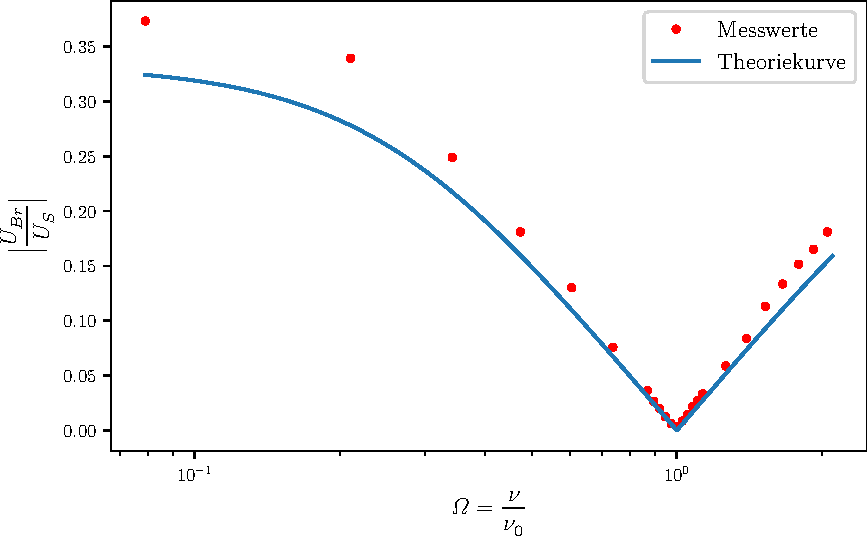
\includegraphics{plot.pdf}
   \caption{TITEL}
   \label{fig:plot}
\end{figure}

\begin{table}
\normalsize
\centering
\sisetup{table-format=4.0}
\begin{tabular}{c c c c}
\toprule
        $2R' \,/\,\si{\ohm}$ & $R' \,/\,\si{\ohm}$ & $R \,/\,\si{\ohm}$ & $C_{4} \,/\, \si{\farad}$ \\
        \midrule
        664 & 332 & 1000 & \num{420e-9} \\
\bottomrule
\end{tabular}
\caption{Text5} 
\label{tab:6}
\end{table}

\noindent
\begin{table}
\normalsize
\centering
\sisetup{table-format=4.0}
\begin{tabular}{c c c c}
\toprule
        $U_{S} \,/\,\si{\milli\volt}$ & $U_{Br} \,/\,\si{\milli\volt}$ & $\upOmega$ & $\nu \,/\, \si{\henry}$ \\
        \midrule
        2500 & 1320 &           0.0789 & 30 \\
        2500 & 1200 &           0.2105 & 80 \\
        2500 & 880 &            0.3221 & 130 \\
        2500 & 640 &            0.4737 & 180 \\
        2500 & 460 &            0.6053 & 230 \\
        2500 & 268 &            0.7368 & 280 \\
        2500 & 128 &            0.8684 & 330 \\
        2500 & 94.4 &           0.8947 & 340 \\
        2500 & 70.4 &           0.9211 & 350 \\
        2500 & 44.0 &           0.9474 & 360 \\
        2500 & 21.6 &           0.9737 & 370 \\
        2500 & 13.6 &           1 & 380 \\   
        2500 & 30 &             1.0263 & 390 \\
        2500 & 52 &             1.0526 & 400 \\
        2500 & 78 &             1.0789 & 410 \\
        2500 & 96 &             1.1053 & 420 \\
        2500 & 118 &            1.1316 & 430 \\
        2500 & 208 &            1.2631 & 480 \\
        2500 & 296 &            1.3947 & 530 \\
        2500 & 400 &            1.5263 & 580 \\
        2500 & 472 &            1.6579 & 630 \\
        2500 & 536 &            1.7894 & 680 \\
        2500 & 584 &            1.9210 & 730 \\
        2500 & 640 &            2.0526 & 780 \\
        
\bottomrule
\end{tabular}
\caption{Text5} 
\label{tab:7}
\end{table}





